\documentclass[11pt, oneside]{article}   	% use "amsart" instead of "article" for AMSLaTeX format
\usepackage{geometry}                		% See geometry.pdf to learn the layout options. There are lots.
\geometry{letterpaper}                   		% ... or a4paper or a5paper or ... 
%\geometry{landscape}                		% Activate for for rotated page geometry
%\usepackage[parfill]{parskip}    		% Activate to begin paragraphs with an empty line rather than an indent
\usepackage{graphicx}				% Use pdf, png, jpg, or eps§ with pdflatex; use eps in DVI mode
								% TeX will automatically convert eps --> pdf in pdflatex		
\usepackage{amssymb}
\usepackage{pdfpages}
\usepackage{booktabs}
\title{FIT2014 - Theory Of Computation}
\author{James Austin}
%\date{}							% Activate to display a given date or no date

\begin{document}
\maketitle
\section{Lecture 1}

\begin{itemize}
\item Natural Languages, English, Chinese, French, Auslan, etc.
\item Programming Languages
\item Mathematics
\item State Diagrams
\item Music
\item Feynman Diagrams
\end{itemize}

Components of language include an alphabet, which are the basic elements that a language is made up of. This is a set of letters of characters. The rules (or grammar) tell you what words belong to the language. They are also the syntax. The meaning of the language is the semantics.

A word is a finite string of characters belonging to the language, while a language is a set of words. For english, the alphabet is a, b, c ... z A B ... Z. It also includes English, punctuation marks and blank space. While the words is in a standard dictionary aardvark, zygote, woot. An empty word is 

For Java, the alphabet is unicode characters, while the words are programs. 

If we have a language that is made of a and b, the words are a b ab abbb bab.... A lot of these words can be expressed by $a^2$.

Even-Even - All the strings that contain an even number of a's and an even number of b's. IE, aa, bb, aaaa,aa,bb,

Palindromes - All the strings which are the same if they are spelt backwards. IE, a, b, aa, bb, aaa,aba, bbb

Double word - All the strings are formed by two copies of a string joined together. IE, aa, bb, aaaa, abab, baba.

Symbols\\
\begin{itemize}
\item $\subset$ Subset
\item $\subseteq$ Subset Equals
\item $\in$ Contains 
\item $\epsilon$      Empty Word 
\item $\phi$ Empty Language
\end{itemize}
Definition: Specifies the precise meaning of certain things
Theorem: A mathematical statement that has been proved to be true. Has some close, but less significant relatives in Proposition and Lemma.
Proof: A step-by-step argument that establishes, logically and with certainty, that something is true.

Existential statements: Statements that require one suitable example for a proof (There exists a palindrome in English).
Universal Statement: Statements where you need to cover every possible case. One way is to go through every possibility in turn and check each one. However the number of things to check may be huge, or infinite. So usually we want to reason in a way can apple to many different possibilities at once.

\section{Lecture 2 - Propositional Logic}

A proposition is a statement which is either true or false. IE, 2 + 2 = 4, or The moon is made of cheese. This statement is false, or Vote for Mickey Mouse, are not propositions.

\subsection{Connectives}
\subsubsection{Negation}

Symbol: $\neg$

$P$: I have three children.\\
$\neg P$: I do not have three children

% Requires the booktabs if the memoir class is not being used
\begin{table}[htbp]
   \centering
   %\topcaption{Table captions are better up top} % requires the topcapt package
   \begin{tabular}{@{} c|c @{}} % Column formatting, @{} suppresses leading/trailing space
      $P$ & $\neg$ P\\
      \midrule
      F      & T\\
      T       & F \\
   \end{tabular}
   \label{tab:booktabs}
\end{table}
\subsubsection{Conjuction (and)}
Symbol: \& or $\wedge$

P: This subject is interesting.
Q: I am tired.
P\textasciicircum Q : This subject is interesting and I'm tired. This subject is interesting although I am tried. This subject is interesting but I am tired.

\begin{table}[htbp]
   \centering
   %\topcaption{Table captions are better up top} % requires the topcapt package
   \begin{tabular}{@{} cc|c @{}} % Column formatting, @{} suppresses leading/trailing space
      $P$ & Q & P \& Q\\
      \midrule
      F & F & F\\
      F & T & F\\
      T & F & F\\
      T & T & T\\
   \end{tabular}
   \label{tab:booktabs}
\end{table}

\subsubsection{Disjunction (Or)}
Symbol: $\vee$

P: Sue is a football player
Q: Bob is lazy.
P $\vee$ Q: Sure is a football player or Bob is lazy.

\begin{table}[htbp]
   \centering
   %\topcaption{Table captions are better up top} % requires the topcapt package
   \begin{tabular}{@{} cc|c @{}} % Column formatting, @{} suppresses leading/trailing space
      $P$ & Q & P \& Q\\
      \midrule
      F & F & F\\
      F & T & T\\
      T & F & T\\
      T & T & T\\
   \end{tabular}
   \label{tab:booktabs}
\end{table}

\subsubsection{Conditional}
Symbol: $\Rightarrow$

$P$: It is tuesday.
$Q$: We are in Belgium
$P\Rightarrow Q$
If it is Tuesday then we are in Belgium.\\
It's being Tuesday implies we are in Belgium.\\
It's Tuesday only if we are in Belgium.\\
It's being Tuesday is sufficient for us to be in Belgium.\\

\begin{table}[htbp]
   \centering
   %\topcaption{Table captions are better up top} % requires the topcapt package
   \begin{tabular}{@{} cc|c @{}} % Column formatting, @{} suppresses leading/trailing space
      $P$ & $Q$ & $P \Rightarrow Q$ \\
      \midrule
      F & F & T\\
      F & T & T\\
      T & F & F\\
      T & T & T\\
   \end{tabular}
   \label{tab:booktabs}
\end{table}


\subsubsection{Biconditional}
Symbol: $\Leftrightarrow$

$P$: It will rain tomorrow.\\
$Q$: I will wear a raincoat tomorrow.\\
$P \Leftrightarrow Q$: I will wear a raincoat tomorrow if and only if it rains.
\begin{table}[htbp]
   \centering
   %\topcaption{Table captions are better up top} % requires the topcapt package
   \begin{tabular}{@{} cc|c @{}} % Column formatting, @{} suppresses leading/trailing space
      $P$ & $Q$ & $P \Rightarrow Q$ \\
      \midrule
      F & F & T\\
      F & T & F\\
      T & F & F\\
      T & T & T\\
   \end{tabular}
   \label{tab:booktabs}
\end{table}


\subsection{De Morgan's Laws}

$\neg(P \vee Q) = \neg P \wedge \neg Q$\\
$\neg(P \wedge Q) = \neg P \vee \neg Q$
\\\\
This can be proven using truth tables.

\begin{table}[htbp]
   \centering
   %\topcaption{Table captions are better up top} % requires the topcapt package
   \begin{tabular}{@{} cc|c|c @{}} % Column formatting, @{} suppresses leading/trailing space
      $P$ & $Q$ & $P \vee Q$ & $\neg (P \vee Q)$ \\
      \midrule
      F & F & F & T\\
      F & T & T & F\\
      T & F & T & F\\
      T & T & T & F\\
   \end{tabular}
   \label{tab:booktabs}
\end{table}

\begin{table}[htbp]
   \centering
   %\topcaption{Table captions are better up top} % requires the topcapt package
   \begin{tabular}{@{} cc|c @{}} % Column formatting, @{} suppresses leading/trailing space
      $\neg P$ & $\neg Q$ & $\neg P \wedge \neg Q$\\
      \midrule
      T & T & T\\
      T & F & F\\
      F & T & F\\
      F & F & F\\
   \end{tabular}
   \label{tab:booktabs}
\end{table}

\subsection{Definitions}
\begin{itemize}
\item Tautology - A statement whose interpretation is always true.
\end{itemize}
\subsection{Logically Equivalent}
Logically Equivalent, two statements that have the same truth table. For example:\\ $P \Rightarrow Q$ is logically equal to $\neg P \vee Q$.\\ $P \Leftrightarrow Q$ is logically equal to $(\neg P \vee Q) \wedge (P \vee \neg Q)$.
\subsection{Solving Real Problems}
\includepdf[pages={4,5}]{lect02-handout-6.pdf}


\section{Lecture 3 - Predicate Logic, Prolog}

In predicate logic, there are 3 types of objects, Constant symbols, Function symbols and Individual Variables. Constant symbols are names which refer to exactly one object (like socrates, medusa, 1 or 2). Function symbols relate some objects to exactly one object (motherOf, kingOf, plus, times). They can have complex names. Individual variables are variables which can relate to any object (X, Y).

A term is a logical expression which refers to an object.

The equality symbol (=) is used to state that two objects are the same (IE rebecca = rebecca, fatherOf(john) = henry.

An example of predicate logic is:
\begin{itemize}
\item All men are mortal.
\item Socrates is a man.
\item Thereforce Socrates is mortal.
\end{itemize}
The objects in this example are socrates and set of people, while the properties are man and mortal. 

\subsection{Sentences}

Atomic sentences: A predicate symbol followed by a list of terms in brackets. EG taller(motherOf(claire), mary).
Complex sentences: Atomic sentences joined together by logical connectives man(socrates) $\Rightarrow$ mortal(socrates).

\subsection{Quantification}
Universal quantification means that the statement applies to all objects. 
$\forall$ = For All
\\\\
An example is All Dogs Are Happy:\\
$\forall x (dog(x) \Rightarrow happy(x))$\\\\
No dog is happy/All dogs are unhappy.\\
$\forall x (dog(x) \Rightarrow \neg happy(x))$\\

For statements that apply only about some object, use $\exists$

Some dogs are happy.\\
$\exists X (dog(x) \wedge happy(x))$

Some dogs are not happy.\\
$\exists X (dog(x) \wedge \neg happy(x))$\\\\

These quantifiers are related.

$\neg \forall x$ is equal to $\exists y \neg$\\

"Not all dogs are happy" is the same as "There exists an unhappy dog".

\subsection{More examples}

There is an app which is loved by every student. This means that there is an app X and if Y is a student, then Y loves it.\\
$\exists X (app(X) \wedge \forall Y(student(Y) \Rightarrow loves(Y,X)))$

Every student loves some app. For every student Y there exists an app X that she loves.\\
$\forall Y(student(Y) \Rightarrow \exists X (app(X) \wedge loves(Y,X)))$


\section{Lecture 4 - Proofs}

There is no systemic method for finding proofs for theorems. Discovering proofs is an art as well as a science. There are proofs of many kind, the main being Proof by Construction, Proof by cases, Proof by contradiction, Proof by Induction. Some proofs are a mix of these.

\subsection{Proof by Construction}
Proof by construction is often known as proof by example. It can be used where the theorem asserts the existence of some object with a specific property. In this case you can just give the example and show it has the property.

\subsection{Proof by Cases}

This is also known as proof by exhaustion, or if there are a lot of cases, brute force. First you identify  a number of different cases which cover all possibilities, then prove the theorem for each of these cases. 

\subsection{Proof by Contradiction}

Start by assuming the negation of the statement you want to prove. Deduce from this a contradiction. Therefore the statement must be true.

\section{Lecture 5 - Regular Expressions}

The language with no words is  $\phi$ Empty Language.\\
The language consisting only of the empty words is  $\epsilon$      Empty Word \\
The language \{ w \} consists only of the single word w.\\

Alternatives are indicated by $\cup$, so $1\cup2\cup3\cup4$ is \{1,2,3,4\}.\\

Groupings are indicated by ( ), so the expression $(ab \cup ba)(e \cup g)$ maps to $\{abe,bag,bas,bag\}$

Finite languages consist of a finite number of words, like $\{ababa,abb.,abbaba\}$. \\This maps to the regular expression $abaaba\cup abbbba \cup abbaba$,\\ which maps to $ab(aa \cup bb \cup ba)ba$, \\which maps down to $ab(a \cup b)aha \cup abb(b \cup a)ba$.

The asterisk (*) is called a Kleene Star, which means zero or more times.

$a*$ represents $\{\epsilon, a,aa,aaa,aaaa,...\}$\\
$(ba)*$ represents $\{\epsilon, ba,baba,bababa,babababa,...\}$\\
$ab*$ represents $\{a,ab,abb,abbb,...\}$

See notes for more examples.


\section{Lecture 6}


\section{Lecture 7}


\section{Lecture 8}



\end{document}  